\chapter{Background}\label{chap:background}
The title of this thesis is \textit{\thesisTitle}.
It brings together the domains of Process Science, Predictive Modeling and Deep Learning.
This chapter gives insights into the parts of these topics that will be used and needed throughout the thesis.
This work can be attributed to the domain of Predictive Process Monitoring, which will also be introduced.

\section{Process Science And Process Monitoring}
Process Science, as loosely defined by van der Aalst \cite{Aalst2016}, refers to the \textit{broader discipline that combines knowledge from information technology and knowledge from management sciences to improve and run operational processes}. This means that approaches in this domain tend to be driven by models, such as Six Sigma or Kaizen\todo{source?}.

Central to process science is Business Process Management (BPM) which is squarely aimed at improving operational business performance through the optimization of business processes via their models.
Modeled e.g. with the Business Process Modeling Notation (BPMN) \cite{bpmn2.0}, they are typically very rigid and permit little variation of the workflow. The central element of these notations are the individual steps of which a process is comprised, referred to as \textit{activities}, as also shown in \ref{fig:activity-introduction}.

\begin{figure}
    \centering
    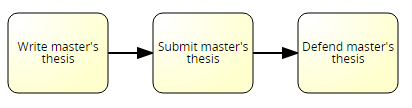
\includegraphics[width=.75\textwidth]{gfx/activity-introduction.png}
    \caption{The yellow boxes and their description are used in BPMN to describe an activity. The arrows denote the control flow in between.}
    \label{fig:activity-introduction}
\end{figure}

With the help of workflow management systems (WFMS), it became possible to embed and enforce structured processes in an organization.
\todo[inline]{taxonomy for variability in processes}

These WMFS also logged execution traces of running process instances. From the analysis of these logs it became obvious that rigid models are not suited equally well for all types of processes. Especially in the insurance and health-care sector, each case tends to be very different from the next \cite{hewelt2016}. This led to the notion that the course of a case strongly depends on the information contained inside it.

\subsection{Case Management}
In settings in which it is common to employ BPM, such as assembly line productions, there is little heterogeneity. As the latter increases, BPMN and other business process modeling notations result in complex and hardly understandable models and thus fail their purpose. As previously mentioned, this tends to occur in domains where the case trajectory is highly dependant on information contained inside it.

The fact that this type of process is data-driven led to the creation of the \textit{case folder} - a directory central to a case, describing its current state. In Case Management, the process acts on the data contained inside this folder, making it have a direct impact on the course of a case. In contrast to BPM, the formalization of Case Management and the subsequent creation of modeling languages has only just begun. Notable developments include the Case Management Modeling Notation \cite{web:cmmn} as well as the Chimera approach \cite{hewelt2016}.
\todo[inline]{graphical illustration of case}

\subsection{Process Mining}
The logs generated through the users actions gave rise to the discipline of Process Mining, which covers the three steps of model discovery, conformance checking and model enhancement \cite{Aalst2016}. This is enabled through the use of techniques from the area of Data Science, making it possible to understand Process Mining as the link between Data Science and Process Science as in \autoref{fig:process-data-science}. An excerpt from a log is depicted in figure \ref{fig:process-log}.

\begin{figure}
    \centering
    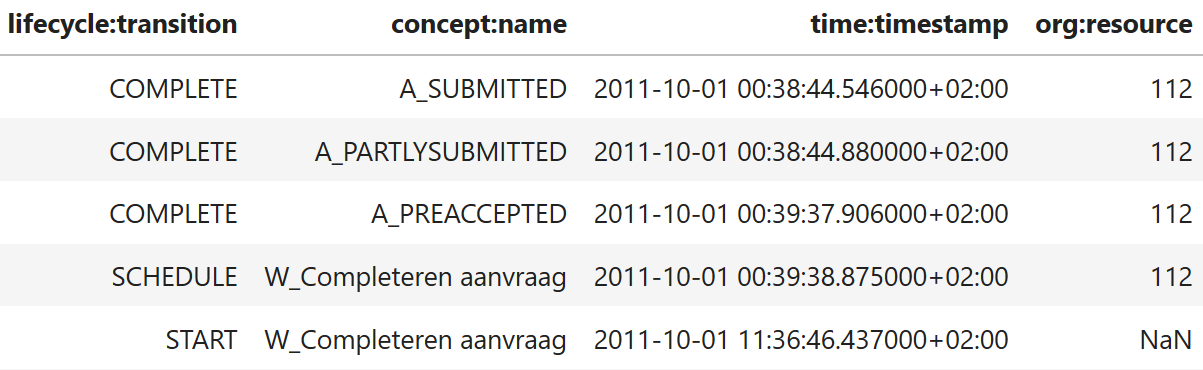
\includegraphics[width=\textwidth]{gfx/process-log}
    \caption{The first entries of an exemplary event log from a case from the BPIC 2011 dataset\cite{BPIC2011}. Each event is associated with data and the column \texttt{concept:name} corresponds to the activity title.}
    \label{fig:process-log}
\end{figure}

\subsection{Predictive Process Monitoring}
In parallel to this development, WFMS already permitted the unstructured execution of processes, empowering the user to make the best choice about which activity to do next. 
As Process Mining is concerned with data-driven process discovery and optimization only on offline data, a possibility to act on case developments in real-time is desirable. Commonly referred to as \textit{Predictive Process Monitoring} \cite{francescomarino2015, schoenig2018}, the application of predictive analytics on running and thus incomplete case logs fulfills this need. It is also visualized in \autoref{fig:process-data-science}.

\begin{figure}
    \centering
    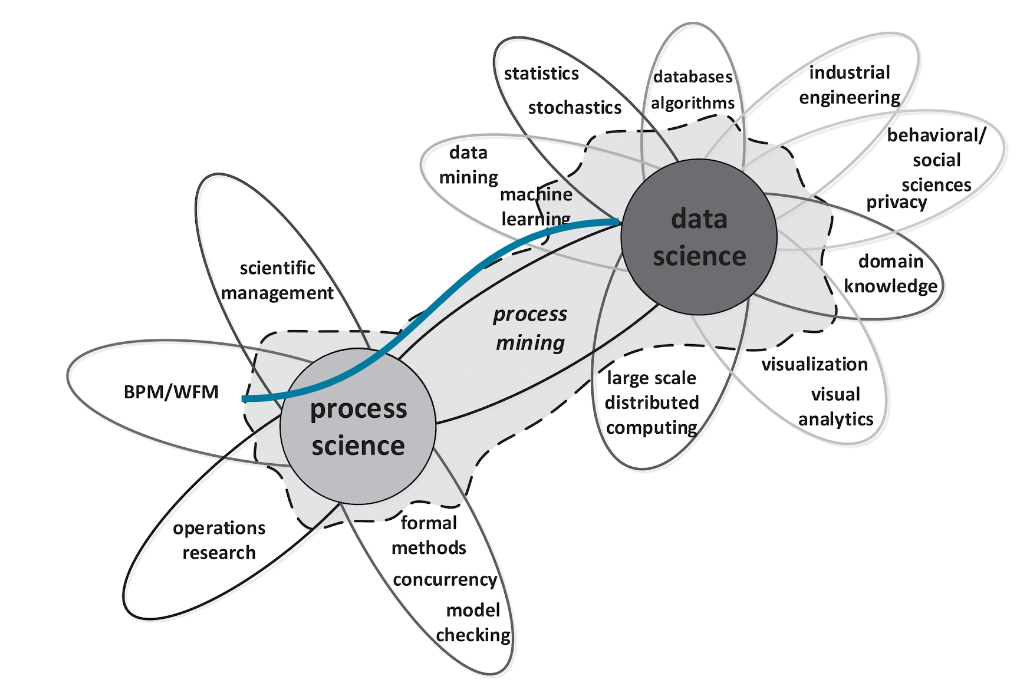
\includegraphics[width=\textwidth]{gfx/process-data-science.png}
    \caption{Process Mining can be understood as the bridge between Process Science and Data Science \cite[p.18]{Aalst2016}. The blue line symbolizes the domains that Predictive Process Monitoring brings together.}
    \label{fig:process-data-science}
\end{figure}

Instead of revolving around models, this discipline is concerned with predicting certain characteristics of the running case that lie in its future. This allows to answer questions such as:

\begin{itemize}
    \item Will I still meet my service level agreement?
    \item Will we be able to deliver the package in within our 3-hour target?
    \item How long is this case still going to take?
    \item What is going to be the next step?
\end{itemize}

The answers to such questions can give case workers the opportunity to intervene if a case takes an unwanted course or might fail to meet KPI requirements. Furthermore, this approach only requires sufficient amounts of historical case executions, but no model. While it can certainly be a useful addition, it is not needed. 

%\begin{figure}
%	\centering
%	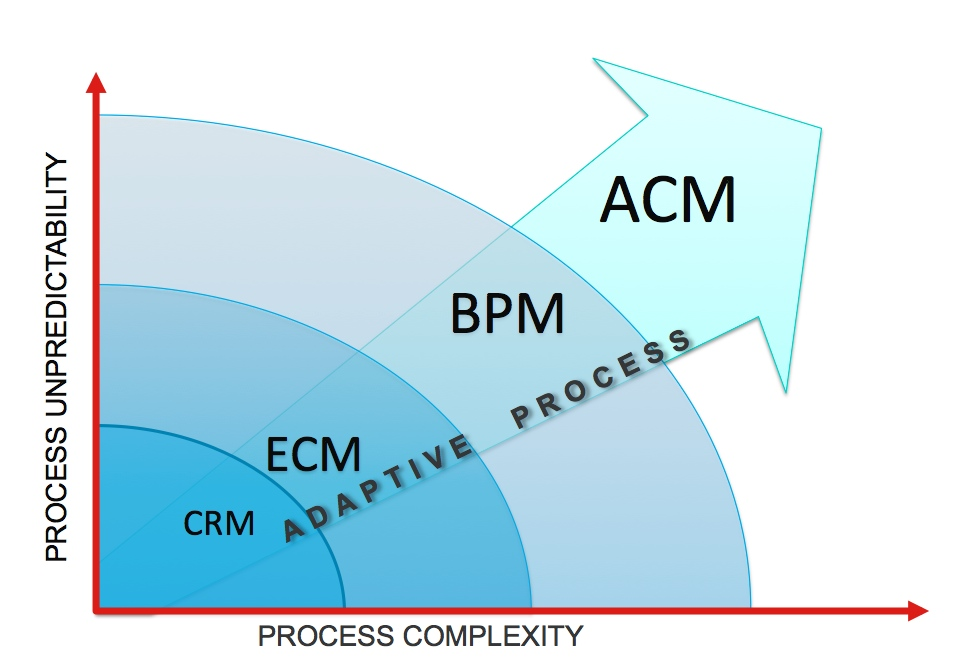
\includegraphics[width=\textwidth]{gfx/acm-reasoning}
%	\caption{https://acmisis.wordpress.com/what-is-adaptive-case-management-acm/}
%	\label{fig:why-acm}
%\end{figure}

\section{Predictive Modeling}
\subsection{Subsequence Mining}

\section{Predictive Modeling}
\subsection{Knowledge Discovery in Databases}
\begin{figure}
	\centering
	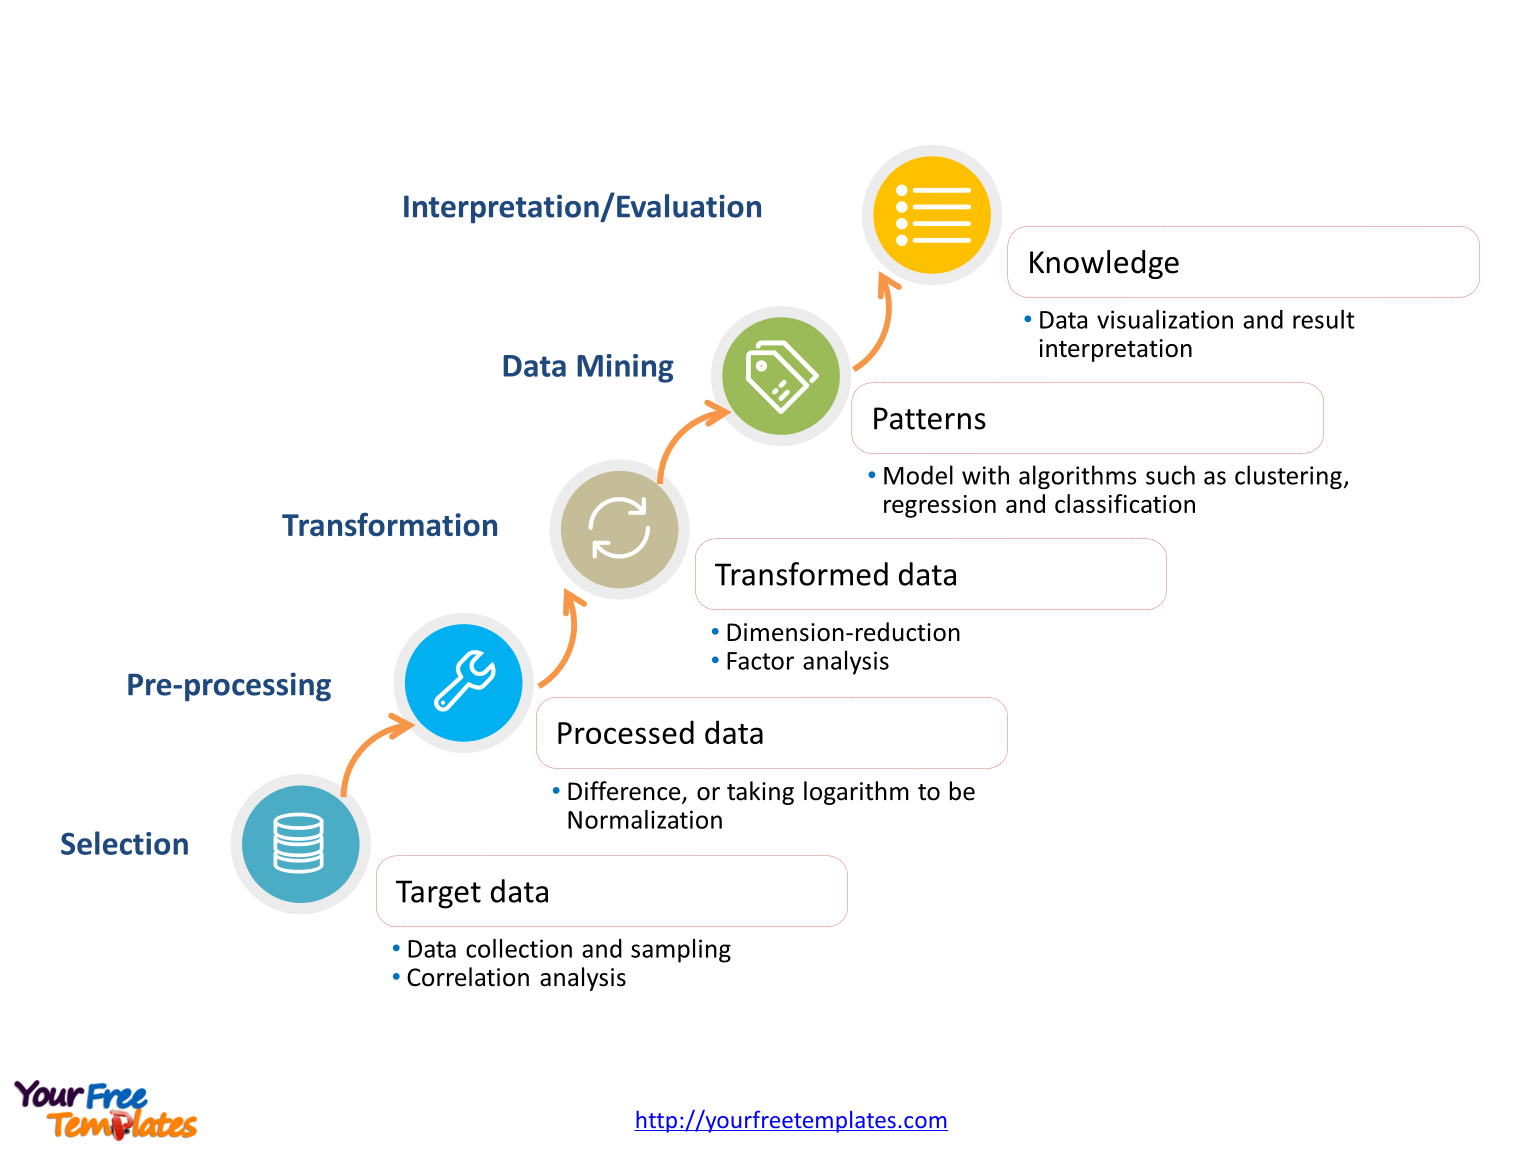
\includegraphics[width=\textwidth]{gfx/kdd_process}
	\caption{The process for \textit{Knowledge Discovery in Databases}}
	\label{fig:kdd_process}
\end{figure}
Predictive analytics is a lot about model training, and the rough outline of necessary steps necessary to train a model is listed here:
\begin{enumerate}
	\item Determine the \textit{target} variable, it is the variable that is supposed to be predicted
	\item Preprocess the dataset. This can mean introducing one-hot encodings, normalized values, but also basic data quality assurance such as null value elimination. Feature engineering can also happen at this step.
	\item Partition the dataset into two parts. One part is set aside for model performance verification, as there the actual target variable value is known. This is commonly referred to as the \textit{test set}, while the remainder is called the \textit{training set}.
	\item Train the model on the training set. Models are trained multiple times with different hyper-parameters to find the optimum configuration with respect to prediction accuracy on the test set. Hyper-parameters are model-specific values such as cutoff-thresholds that have impact on model performance.
\end{enumerate}

\subsection{Language Modeling}
\subsubsection{Sequence-to-Sequence prediction}
\subsubsection{Sequence-to-word prediction}

\subsection{Popular feature engineering techniques}
\subsubsection{Sliding Window}
\subsubsection{N-gram}
\subsubsection{Bag-Of-Words}
\subsubsection{Learned features, word2vec}
Strictly piecewise\\
subsequences, embedding
PrefixSpan

\subsection{Neural networks}
\subsubsection{RNN}
\subsubsection{LSTM memory}